\documentclass{beamer}
\usetheme{Boadilla}
\usepackage{xcolor}
\definecolor{col1}{rgb}{0.5,0.7,0.8}
\definecolor{col2}{rgb}{0.5,0.7,0.5}
\usepackage[english]{babel}
\usepackage{biblatex}
\addbibresource{references.bib}



\title{Time Series Modeling and Prediction of All-Transaction House Price Index (HPI) in Connecticut}\\
\author{Jingqian Xu}

\date{\today}

\begin{document}

\begin{frame}
\titlepage
\end{frame}

\begin{frame}
\frametitle{Outlines}
\begin{itemize}
    \item Background Information
    \item Description of Data
    \item Description of Objective
    \item Data Analysis
    \begin{itemize}
        \item Exploratory Data Analysis (EDA)
        \item Model Construction
        \item Estimation of Model
        \item Diagnostic Checking
        \item Prediction
    \end{itemize}
    \item Limitations of Analysis
    \item Summary
    \item Reference 
    
\end{itemize}
\end{frame}

\begin{frame}
\frametitle{Background Information}
\begin{figure}
    \centering
    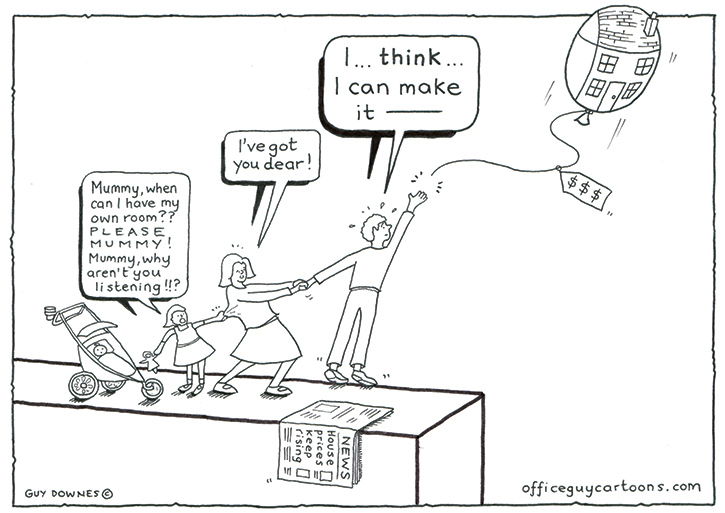
\includegraphics[scale = 0.25]{CARTON.jpg}
\end{figure}


The rise in home prices year-over-year for November 2021 is \begin{huge}
\textbf{\textcolor{col1}{17.5\%}}
\end{huge} as reported by the FHFA on Jan.25, 2022.

In September 2022, home prices in Connecticut were up  \begin{huge}
\textbf{\textcolor{col2}{10.0\%}}
\end{huge} compared to last year, selling for a median price of \$365,400. 
\end{frame}

\begin{frame}
\frametitle{Background Information}
    \begin{itemize}
    
    \item Housing Price Index (HPI) from The U.S. Federal Housing Finance Agency (FHFA) is the reliable house price indexes that measure changes in single-family home values based on data from all 50 states and over 400 American cities that extend back to the mid-1970s.
    
    \item HPI incorporates tens of millions of home sales, offers insights about house price fluctuations and serves as a timely, accurate indicator of house price trend at various geographic levels.
    
    \item Real house price at the State level are driven by fundamentals such as real per capital disposable income, net borrowing cost and State level population growth \cite{1}.
    
    \end{itemize}
\end{frame}

\begin{frame}
\frametitle{Background Information}
\begin{figure}
    \includegraphics[scale = 0.25]{HPIinUS.png}
    \caption{2022 Q2 All-Transactions House Price Index by State\cite{2}}
    \printbibliography
\end{figure}
    Although HPI in Connecticut increases by 7 times since 1980, Connecticut is one of states having less HPI increment in the New England.
\end{frame}

\begin{frame}
\frametitle{Description of Data}
\begin{itemize}
    \item The HPI data resource is U.S. Federal Housing Finance Agency (FHFA\textregistered)\cite{2}.
    \item The explanatory economic indicators (per captia personal income in Connecticut\cite{3}, population growth rate in Connecticut and 10-Year Real Interest Rate in the U.S.\cite{4}) we may use comes from the Federal Reserve Economic Data(FRED\textregistered). 
    \item The file CTSTHPI.csv contains quarterly time series data of HPI and the date they are collected. HPI is not seasonally adjusted, and the first record of HPI is 100 in the first quarter of 1980.
    \item Total 190 HPI observations are collected from January 1st 1975 to April 1st 2022 without missing value. 
\end{itemize}
\end{frame}

\begin{frame}
\frametitle{Description of Objective}
\begin{enumerate}
    \item Conduct Exploratory Data Analysis (EDA) of raw HPI data and find the proper type of time series models to fit the pattern of HPI well and explain the variability of HPI well.
    \begin{itemize}
        \item The first type of model are those have ${X_t}$ but no other explanatory variables, such as models from ARIMA family.
        \item The second type of model is regression model with exogenous explainable variables, such as ARIMAX model.
    \end{itemize}
    \item Conduct model selection, estimate the model parameters, check the model adequacy and make prediction.
    \item Future HPI prediction, interpretation of prediction result and draw some insightful conclusion.
\end{enumerate}
    

\end{frame}

\begin{frame}
\frametitle{Exploratory Data Analysis (EDA)}
\begin{figure}
\centering
\includegraphics[scale = 0.5]{Trend}
\caption{All-Transactions House Price Index for Connecticut from 1975 to 2022}
\end{figure}
We find the seasonality of HPI, and it repeats its pattern around every 20 years. HPI increases in the first decade and drop in another half. Also, the HPI in Connecticut keeps increasing from early 1970s to 2020.
\end{frame}

\begin{frame}
\frametitle{Exploratory Data Analysis (EDA)}
\begin{figure}
    \centering
    \includegraphics[scale = 0.55]{PLOTofAll.png}
    \caption{Time Series for both Response and Exogenous Variables}
    \label{fig:my_labl}
\end{figure}

\end{frame}


\begin{frame}{Exploratory Data Analysis (EDA)}
\begin{figure} 
    \centering
    \includegraphics[scale = 0.55]{CovarianceMatrix.png}
    \caption{Covariance Matrix for Response and Exogenous Variables}
    \label{fig:my_labl}
\end{figure}
\end{frame}

\begin{frame}
\frametitle{Data Pre-processing}
\begin{itemize}
    \item Checking the missing value of raw data and impute missing values.
    \item The time series of economic and demographic data having various time interval. The per capital disposable income and population in the Connecticut is yearly collected from 1975.1.1 to 2021.1.1 and from 1900.12.1 to 2021.12.1 separately. We will unify the time interval for modeling purpose.
    \item 10-year interest rate is monthly collected from 1982.1.1 to 2022.10.1. We will use rolling average method to transform the monthly data into annual data. Similarly, we will transform quarterly HPI data into annual data.
\end{itemize}
\end{frame}





\begin{frame}
\frametitle{Model Construction}
\begin{figure}
\includegraphics[scale=0.4]{ACFs.png}
\caption{ACF Plot Under different Order}
\end{figure}
\end{frame}

\begin{frame}{Model Construction}
\begin{itemize}
    \item Time series $X_{t}$ is said to follow an integrated autoregressive-moving average model $(ARIMA)$ if the $d$ th difference ${W_{t}} = \nabla ^dX_{t}$ is a stationary $ARMA$ process. If $W_{t}$ is $ARMA(p,q)$, we say that ${X_{t}}$ is $ARIMA(p,d,q)$.
    \item The differencing operation on an arbitrary time series $X_{t}$ is defined as:\[\nabla X_{t} = X_{t}-X_{t-1}\] \[\nabla^2X_{t} =\nabla(\nabla X_{t}) = (X_{t}-X_{t-1})- (X_{t-1}-X_{t-2})\]
    \item The $ARIMA(p,d,q)$ is expressed as: \[\nabla ^dX_{t} =\theta_{0}+\sum_{i=1}^{p}\phi_{i}\nabla^dX_{t-i}+a_{t}-\sum_{i=1}^{q}\theta_{i}a_{t-1}\] \[a_{t} \sim i.i.d.N(0,\sigma^2),\sigma^2<\infty\].
    
\end{itemize}
 
\end{frame}
\begin{frame}{Model Construction}
\begin{itemize}
    \item The time series is not stationary since the noticeable increment trend is detected and ACF slowly decays in the following raw data ACF plot. So, we transform the time series into stationary time series by using the first order difference and second order difference.
    \item The second order difference is helpful and ACFs after lag 5 basically lay inside the confidence limit. So, we consider the d in our model as 2. Also, we may consider MA (5) model based on the ACF plot. Also, we draw the time series plot and PACF plot to identify p and q. Based on the plots below, we may consider AR (2) model. 

    
\end{itemize}
    
\end{frame}


\begin{frame}{Model Fitting}
\begin{itemize}
    \item Above procedure is rough. So, we consider a more data driven approach and select best model based on the best in-sample model selection criteria (e.g. BIC) So, we find $ARIMA(2,2,2)$ model has the lowest BIC equal to 5.5832. It's written as: \[\nabla ^2X_{t} =\theta_{0}+\sum_{i=1}^{2}\phi_{i}\nabla^2X_{t-i}+a_{t}-\sum_{i=1}^{2}\theta_{i}a_{t-1}\].
    \item We use the conditional least squared estimation to get the fitted model: 
    \[\nabla^2X_{t} =-0.4802\nabla^2X_{t-1}-0.6436\nabla^2X_{t-2}+a_{t}+1.6236a_{t-1}-0.6792a_{t-2}\]
    \item Is the model adequate?
\end{itemize}
    
\end{frame}
\begin{frame}{Diagnostic Checking}
\begin{figure}
    \centering
    \includegraphics[scale = 0.4]{ModelChecking.png}
    \label{fig:my_label}
\end{figure}
Since the ACFs of residual are within the confidence limit, normality of residual is valid and all p-values of Ljung-Box statistic are larger than critical value, the $ARIMA(2,2,2)$ model is adequate.
    
\end{frame}
\begin{frame}{Prediction}
\begin{figure}
    \centering
    \includegraphics[scale = 0.45]{PredictionO2.png}
    \label{fig:my_label}
\end{figure}
The time interval of in-sample prediction ranges from the Q4 of 2019 to the Q2 of 2022. The out-of-sample prediction is 10 steps ahead namely from Q3 2022 to Q1 2025.
    
\end{frame}

\begin{frame}{Prediction}
Now, we convert double difference data into actual number.
\begin{figure}
    \centering
    \includegraphics[scale = 0.45]{PREDICTION.png}
    \label{fig:my_label}
\end{figure}
Is our prediction result reliable?
\end{frame}


\begin{frame}
\frametitle{ARIMAX Model Construction}
\begin{item}
\item $ARIMAX$ models refer to $ARMA$ models with exogenous predictors. Suppose the data consist of an observed time series $Y_{t}$ along with $r$ deterministic, exogenous predictors $Z_{t,j},j=1,...,r$. We have following $ARIMAX$ model.
\[Y_{t} =\beta_{0}+\theta_{1}Z_{t,1}+\theta_{r}Z_{t,r}+X_{t}\]
\[\phi(B)X_{t}=\theta(B)a_{t}\]
Where $a_{t}\simWN(0,\sigma^2)$, only $Y_{t}$ and $Z_{t,j},j=1,2,3$ are observed. \\

\\Since the con-linearity is observed from covariance matrix for response and exogenous variables. We centralized our response and residuals.

\end{item}
\end{frame}

\begin{frame}
\frametitle{ARIMAX Model Construction}
\begin{figure}
    \centering
    \includegraphics[scale = 0.7]{ACFofResidual.png}
    \label{fig:my_label}
\end{figure}
The sample PACF plot suggests that an AR(1) or MA(3) could be reasonable fit to the residuals $X_{t}$. Also, we choose order d = 2 as we do before. However, the selection method is rough and we get $ARIMAX(1,2,2)$ based on BIC.
\end{frame}

\begin{frame}
\frametitle{Joint Estimation of ARIMAX model}

Based on the RStudio output, we can write the $ARIMAX(1,2,2)$ model as
\[y_{t} =0.3399z_{t,1}-0.0932z_{t,2}+0.0330z_{t,3}+x_{t}\]
\[\nabla^2x_{t}=0.6753\nabla^2x_{t-1}+a_{t}-0.0001a_{t-1}+1.0000a_{t-2}\]
Where $a_{t}\sim WN(0,\sigma^2)$, lower case $y_{t}$ and $z_{t,j},j=1,2,3$ are centralized observations. \\
\end{frame}

\begin{frame}
\frametitle{Diagnostic Checking of ARIMAX model}
\begin{figure}
    \centering
    \includegraphics[scale = 0.6]{DIAG_ARIMAX122.png}
    \label{fig:my_label}
\end{figure}
For the diagnostic plot above, the $ARIMAX(1,2,2 )$ model is adequate.
\end{frame}

\begin{frame}
\frametitle{Prediction}
\begin{figure}
    \centering
    \includegraphics[scale = 0.45]{ARIMAX_Prediction.png}
    \label{fig:my_label}
\end{figure}
It’s expected that 10-year real interest rates will continue to increase in the near future and ranges from 3.0 to 4.0.
It's estimated that the population will 
exceed 3.7 million in 2020, and approach 3.75 million by 2025.
Supposed the expected per-capita disposable income continue goes up.
\end{frame}

\begin{frame}{Limitation of Analysis}

\begin{itemize}
    \item We find that both model can't capture the increment trend of HPI very well shown in the in-sample prediction.
    \item The model we choose based on BIC may not be the model having the best prediction ability.
    \item We can try another method to remediate the con-linearity in deterministic part of ARIMAX model like the principal component regression (PCR).
    \item The collected data have different length and we have to cut some part of raw data to meet the need of model construction.
\end{itemize}
\end{frame}

\begin{frame}{Summary}
    \begin{enumerate}
        \item ARIMA model shows that the HPI in Connecticut will keep moving upwards from 600 to 750 in the next 10 quarters.It indicates that the single house price in Connecticut is very likely to increase in the next 2.5 years.
        \item Supposed the 10-year real interest rate increase steadily in the next couple of years, population and per-captia disposable income in Connecticut follow its expected increment pattern, the HPI will keep increasing.
        \item Our findings correspond with the former research outcomes: per-captia disposable income, population is positively correlated with HPI, while rate is negatively correlated with HPI.
    \end{enumerate}
\end{frame}

\begin{frame}
\frametitle{Reference}

\begin{thebibliography}{10}
\bibitem{1}
Holly, Sean, M. Hashem Pesaran, and Takashi Yamagata. "A spatio-temporal model of house prices in the USA." Journal of Econometrics 158, no. 1 (2010): 160-173.
\bibitem{2}
U.S. Federal Housing Finance Agency, All-Transactions House Price Index for Connecticut [CTSTHPI], retrieved from FRED, Federal Reserve Bank of St. Louis; https://fred.stlouisfed.org/series/CTSTHPI, November 9, 2022.
\bibitem{3}
U.S. Bureau of Economic Analysis and Federal Reserve Bank of St. Louis, Per Capita Personal Income in Connecticut [CTPCPI], retrieved from FRED, Federal Reserve Bank of St. Louis; https://fred.stlouisfed.org/series/CTPCPI, November 9, 2022.
\bibitem{4}
Federal Reserve Bank of Cleveland, 10-Year Real Interest Rate [REAINTRATREARAT10Y], retrieved from FRED, Federal Reserve Bank of St. Louis; https://fred.stlouisfed.org/series/REAINTRATREARAT10Y, November 9, 2022.

\end{thebibliography}
\end{frame}

\end{document}